\documentclass{beamer}

\usepackage[l2tabu, orthodox]{nag}


% % % % % % % % % %
% MATH
% % % % % % % % % %
\usepackage[fleqn]{amsmath}	% fleqn for left alignment of math blocks (as in classicthesis)
\usepackage{amssymb}
\newcommand{\eq}[1]{\begin{align*}#1\end{align*}}
\newcommand\numberthis{\addtocounter{equation}{1}\tag{\theequation}}


% % % % % % % % % %
% FONTS
% % % % % % % % % %
\usepackage[osf,sc]{mathpazo} % Palatino as the main font
\linespread{1.05}\selectfont % Palatino needs some extra spacing, here 5% extra
%\usepackage[scaled=0.85]{beramono}
\usepackage[euler-digits]{eulervm} % nicer math font


% % % % % % % % % %
% FLOATS, FIGURAES, AND TABLES
% % % % % % % % % %
\usepackage{graphicx} 		% Required for including images
\usepackage{caption}
\captionsetup{font=small} 	% format=hang,
\usepackage{subfig}
\usepackage{tabularx}
\setlength{\extrarowheight}{3pt} % increase table row height
\usepackage{pbox} 			% for linebreaking in cells
\usepackage{multicol, multirow}
\usepackage{tikz}
\usetikzlibrary{fit,arrows,shapes}
\usetikzlibrary{decorations.pathreplacing}



% % % % % % % % % %
% BIBLIOGRAPY
% % % % % % % % % %


\usepackage[
	%backend=biber, %instead of bibtex
	backend=bibtex8,bibencoding=ascii,%
	language=auto,%
	style=numeric-comp,%
	%style=authoryear-comp, % Author 1999, 2010
	%bibstyle=authoryear,dashed=false, % dashed: substitute rep. author with ---
	sorting=nyt, % name, year, title
	maxbibnames=10, % default: 3, et al.
	%backref=true,%
	natbib=true % natbib compatibility mode (\citep and \citet still work)
]{biblatex}
\usepackage{biblatex}
% alternative: \usepackage{natbib}


% % % % % % % % % %
% MISC
% % % % % % % % % %
\usepackage
[
%disable
]{todonotes}
\usepackage[utf8]{inputenc} % allow utf-8 input
\usepackage[T1]{fontenc}    % use 8-bit T1 fonts
\usepackage[english]{babel} % hyphenation, special characters, ...
\usepackage{csquotes}		% recommended with babel for quotes
\usepackage{hyperref}       % hyperlinks
\usepackage{cleveref}		% provides \cref for nice in-document refs
\usepackage{url}            % simple URL typesetting
\usepackage{nicefrac}       % compact symbols for 1/2, etc.
\usepackage
[
activate={true,nocompatibility}, % activate protrusion and expansion
final,						% enable microtype; use "draft" to disable
tracking=true,
kerning=true,
spacing=true,
factor=1100,				% add 10% to the protrusion amount (default: 1000)
stretch=10,					% reduce stretchability (default: 20)
shrink=10					% reduce shrinkability (default: 20)
]
{microtype}
\usepackage{cancel}			% easy cancelling of terms: \cancel{expression}

\usepackage{default}
\usepackage{mlmacros}


\title{Reparametrisation Tricks\\ or\\ How to Differentiate Through Samples from Probability Distributions}
\author{Adam Kosiorek}

\AtBeginSection[]{
	\begin{frame}{Table of Contents}
		\tableofcontents[currentsection]
	\end{frame}
}

\graphicspath{ {figs/} }
\variables{a,d,x,y,z}
\variables{I,W}
\variables[mean]{\mu}
\variables[std]{\sigma}
\probdists{p,q}

\captionsetup[figure]{labelformat=empty}% redefines the caption setup of the figures environment in the beamer class.
\beamertemplatenavigationsymbolsempty

\newcommand{\idx}[1]{^{(#1)}}


\newcommand{\layer}[4][$\sigma$]{% nonlin, inpt, xpos, number
	\node[rectangle, draw] (w#4) at (1.5 + #3, 1) {$\bW^{(#4)}$};
	\node  (z#4) at (1.5 + #3, 0) {$\bz^{(#4)}$};
	\node[rectangle, draw] (s#4) at (1.5 + #3, -1) {#1};
	\node (a#4) at (2.5 + #3, 0) {$\ba^{(#4)}$};

	\draw[->] (#2) to [out=90, in=180](w#4);
	\draw[->] (w#4) to (z#4);
	\draw[->] (z#4) to (s#4);
	\draw[->] (s#4) to [out=0, in=-90] (a#4);	
}

\begin{document}


\begin{frame}
	\titlepage
\end{frame}

\section{A Few Examples}
		
	\begin{frame}{Playing Starcraft}
		\begin{figure}
			\centering
			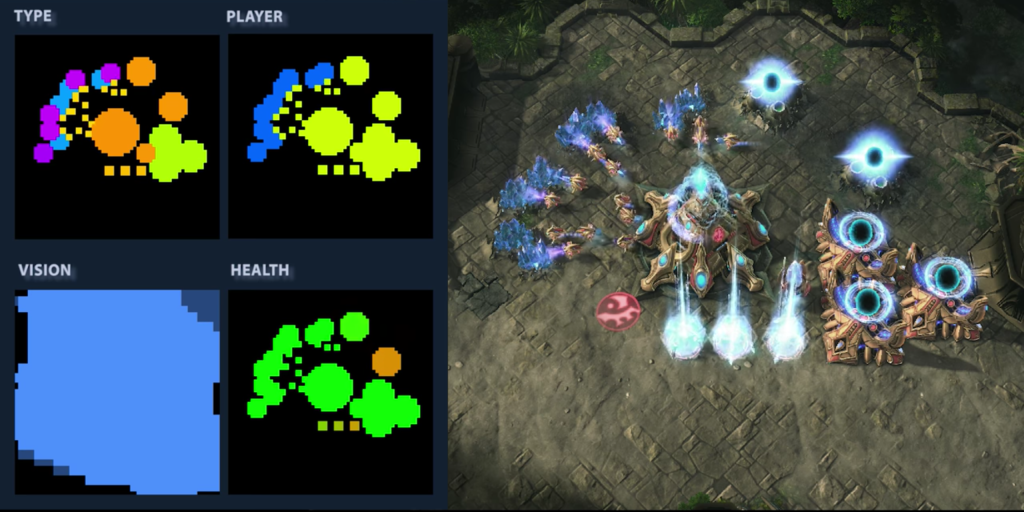
\includegraphics[width=\textwidth]{starcraft}
		\end{figure}

		\begin{equation*}
			\begin{aligned}
				\theta_t &= f_\phi \left( \bxts \right) & \text{compute parameters}\\
				\at &\sim \p{a}{\theta_t} & \text{sample action from a distribution}\\
				R &= R \left( \baTs, \bxTs \right) & \text{compute reward based on actions and states}
			\end{aligned}
		\end{equation*}
	\end{frame}

	\begin{frame}{Alex Kendall's work on uncertainty}
		\begin{figure}
			\centering
			\begin{minipage}{0.45\textwidth}
				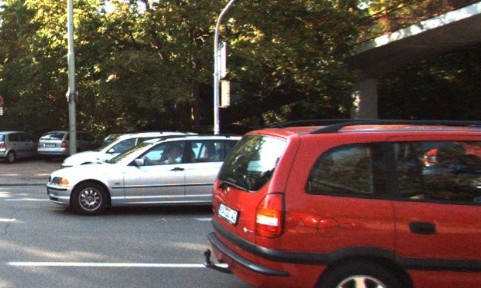
\includegraphics[width=\textwidth]{kendall_rgb}
				\caption{Input image $\bI$}
			\end{minipage}
			\hfill
			\begin{minipage}{0.45\textwidth}
				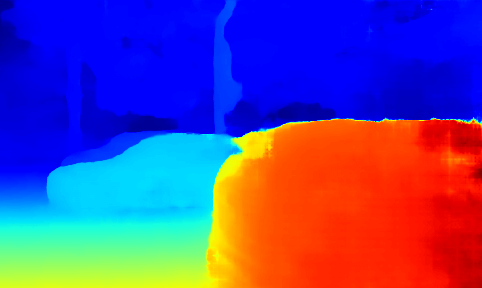
\includegraphics[width=\textwidth]{kendall_depth}
				\caption{Depth estimate $\bd$}
			\end{minipage}
			\hfill
			\begin{minipage}{0.45\textwidth}
				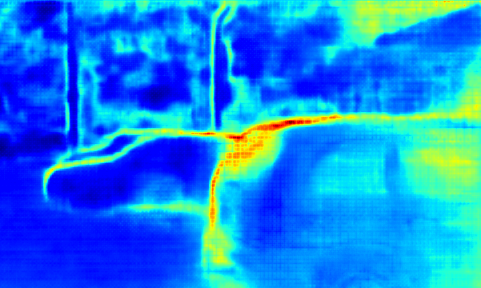
\includegraphics[width=\textwidth]{kendall_uncert}
				\caption{Uncertainty $\bstd^2$}
			\end{minipage}
			\hfill
			\begin{minipage}{0.45\textwidth}
				\begin{equation*}
					\begin{aligned}
						\bmean, \bstd^2 &= f_\phi \left( \bI \right)\\
						\bd &\sim \gauss{\bd \mid \bmean, \bstd^2}
					\end{aligned}
				\end{equation*}
			\end{minipage}
		\end{figure}

	\end{frame}

	\begin{frame}{Stochastic Attractors of Chaotic Systems\\ \textcolor{gray}{\tiny{Neil Dhir, Adam Kosiorek, Michael Osborne, Ingmar Posner}}}
				\begin{figure}
			\centering
			\begin{minipage}{0.45\textwidth}
				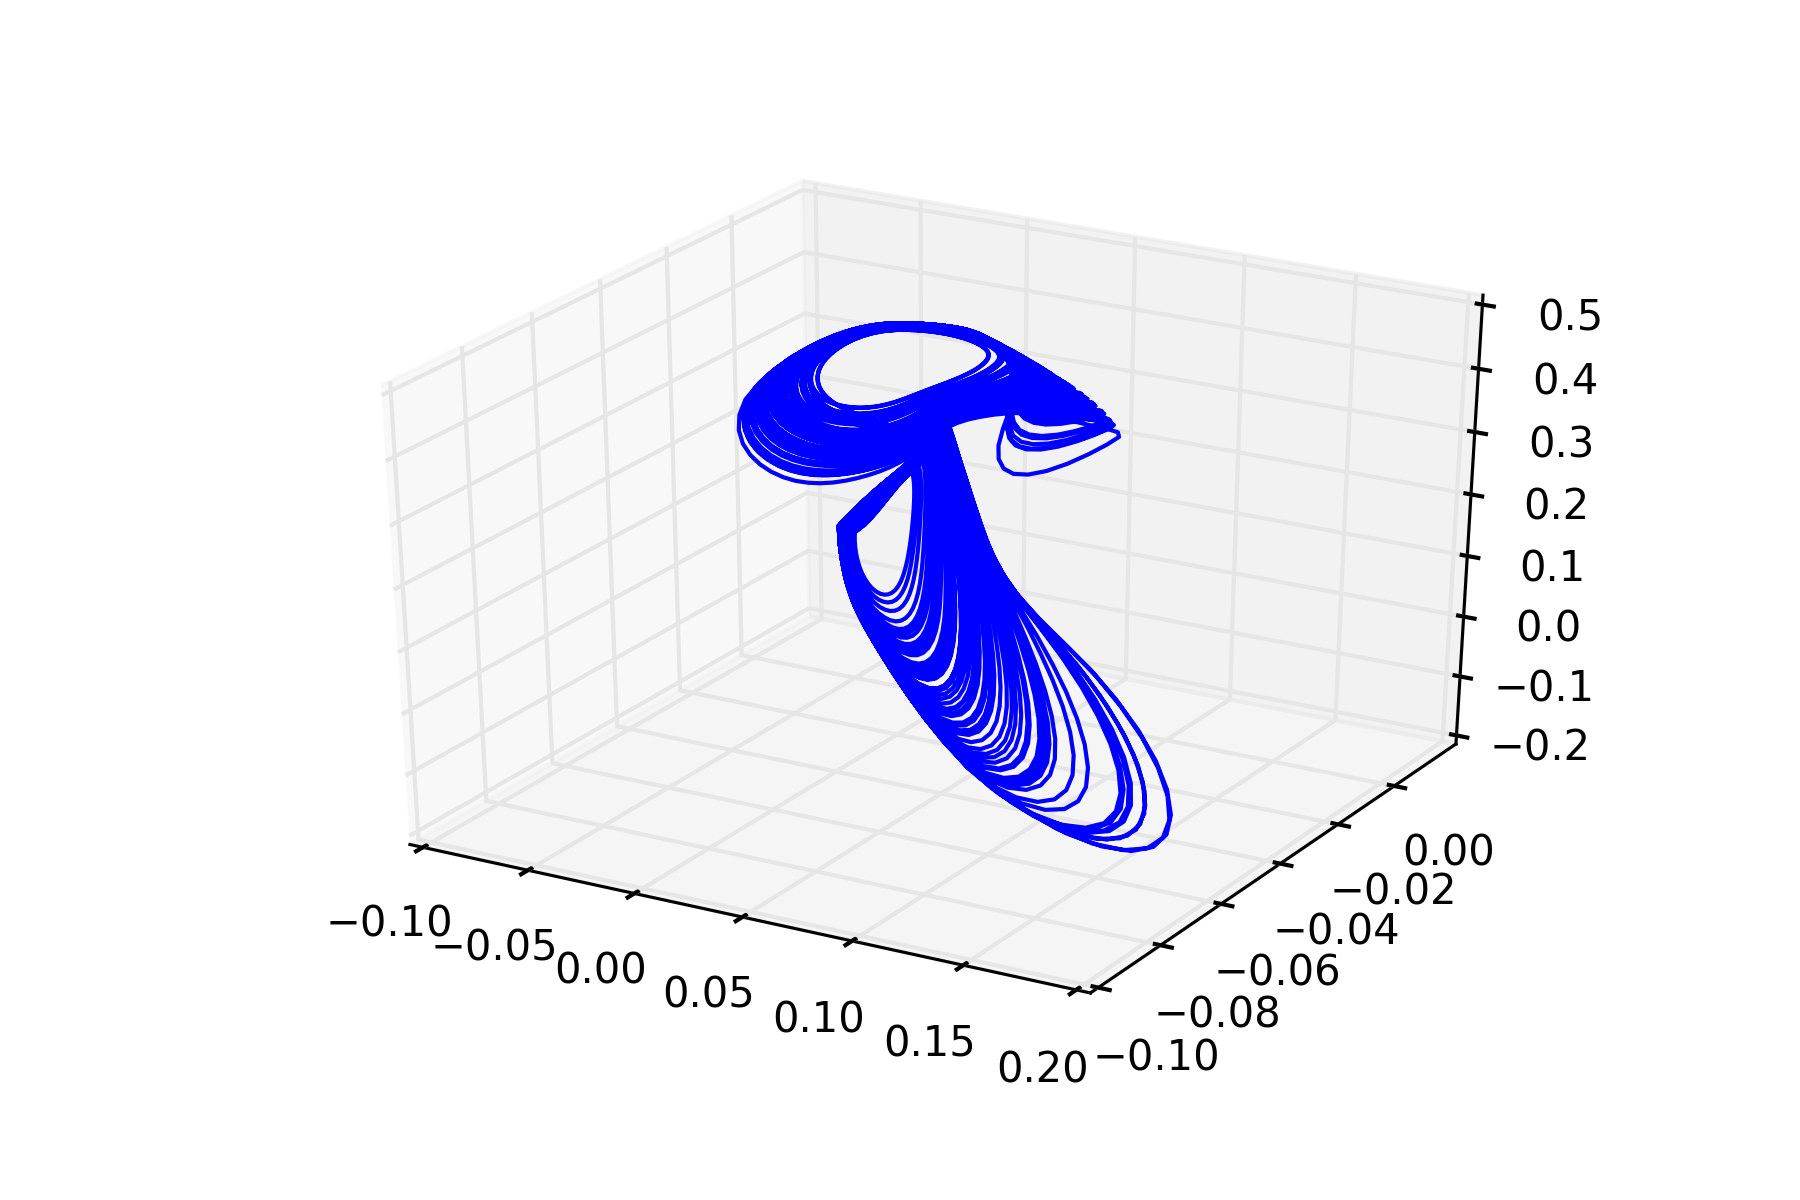
\includegraphics[width=\textwidth]{attractor4}
			\end{minipage}
			\hfill
			\begin{minipage}{0.45\textwidth}
				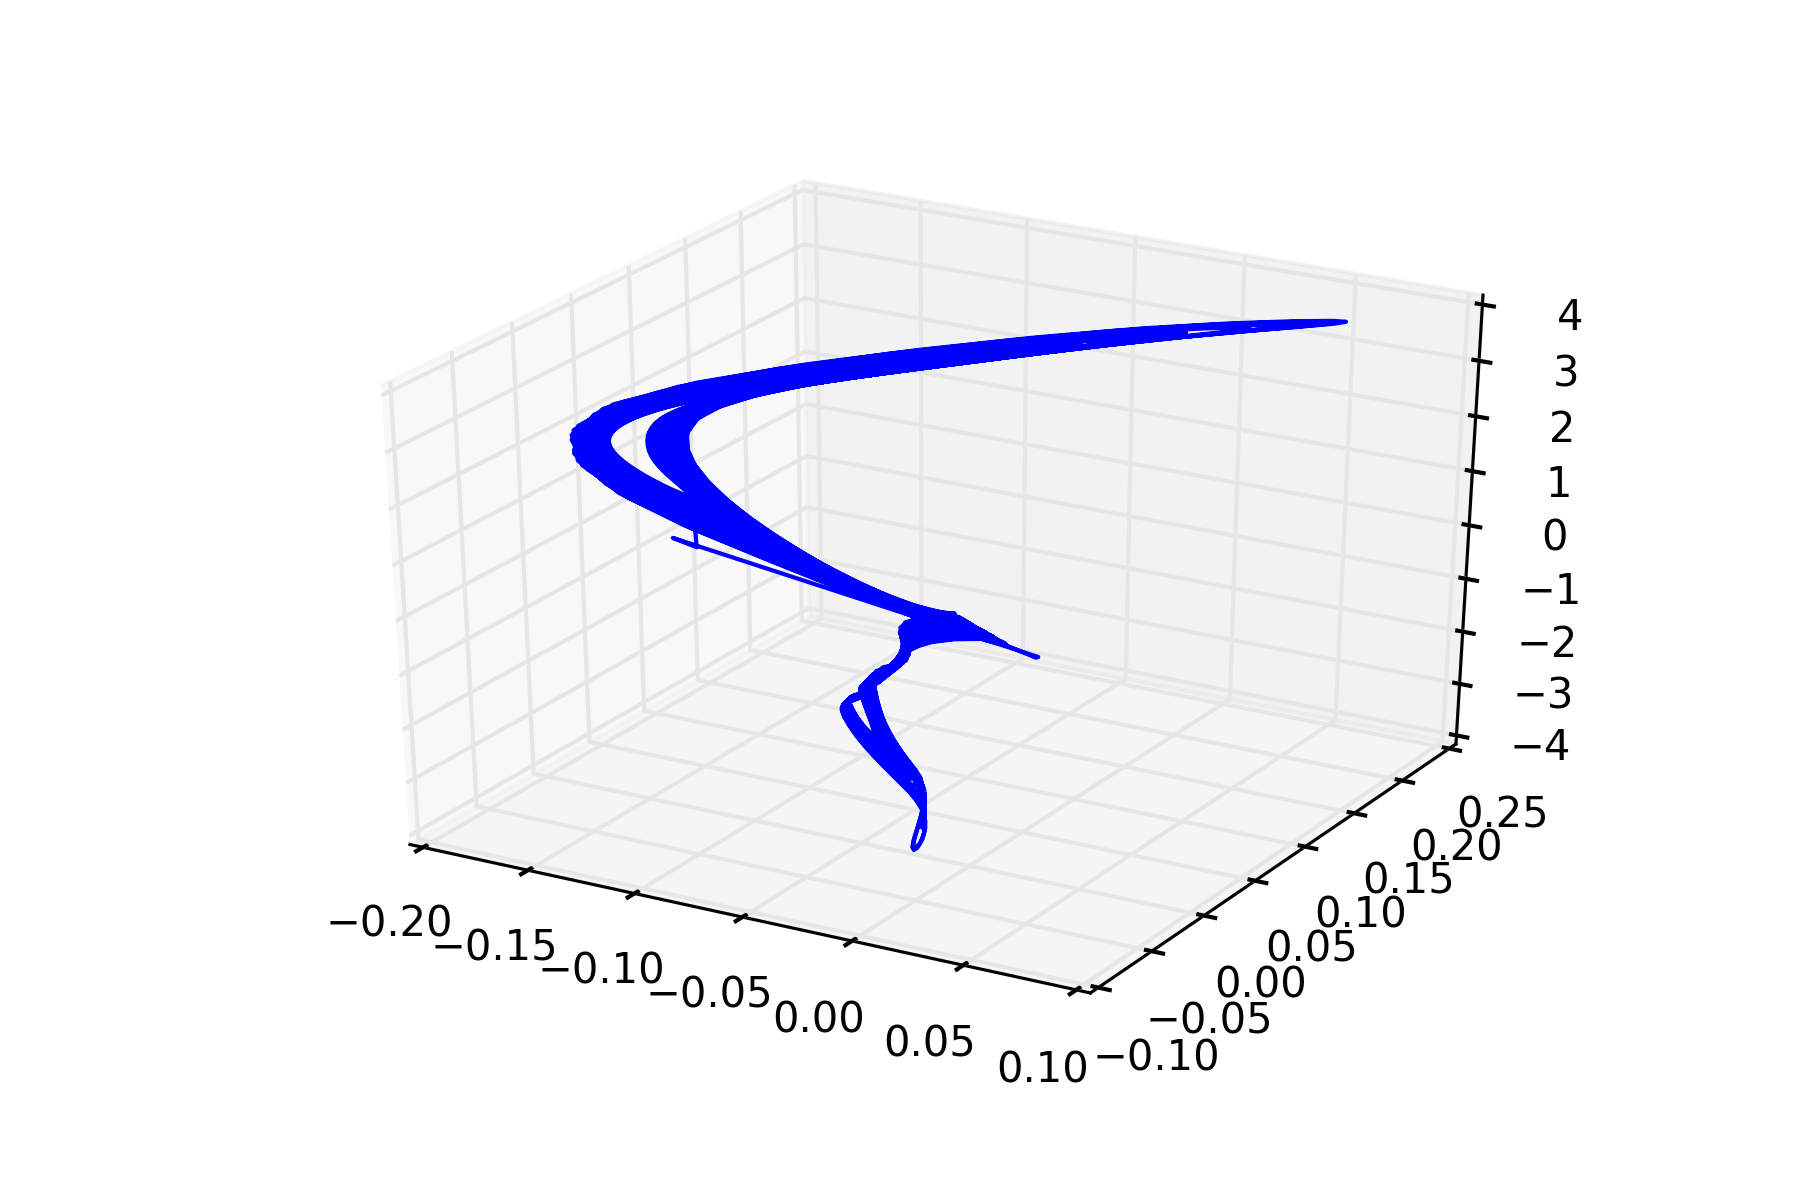
\includegraphics[width=\textwidth]{attractor5}
			\end{minipage}
			\hfill
			\begin{minipage}{0.45\textwidth}
				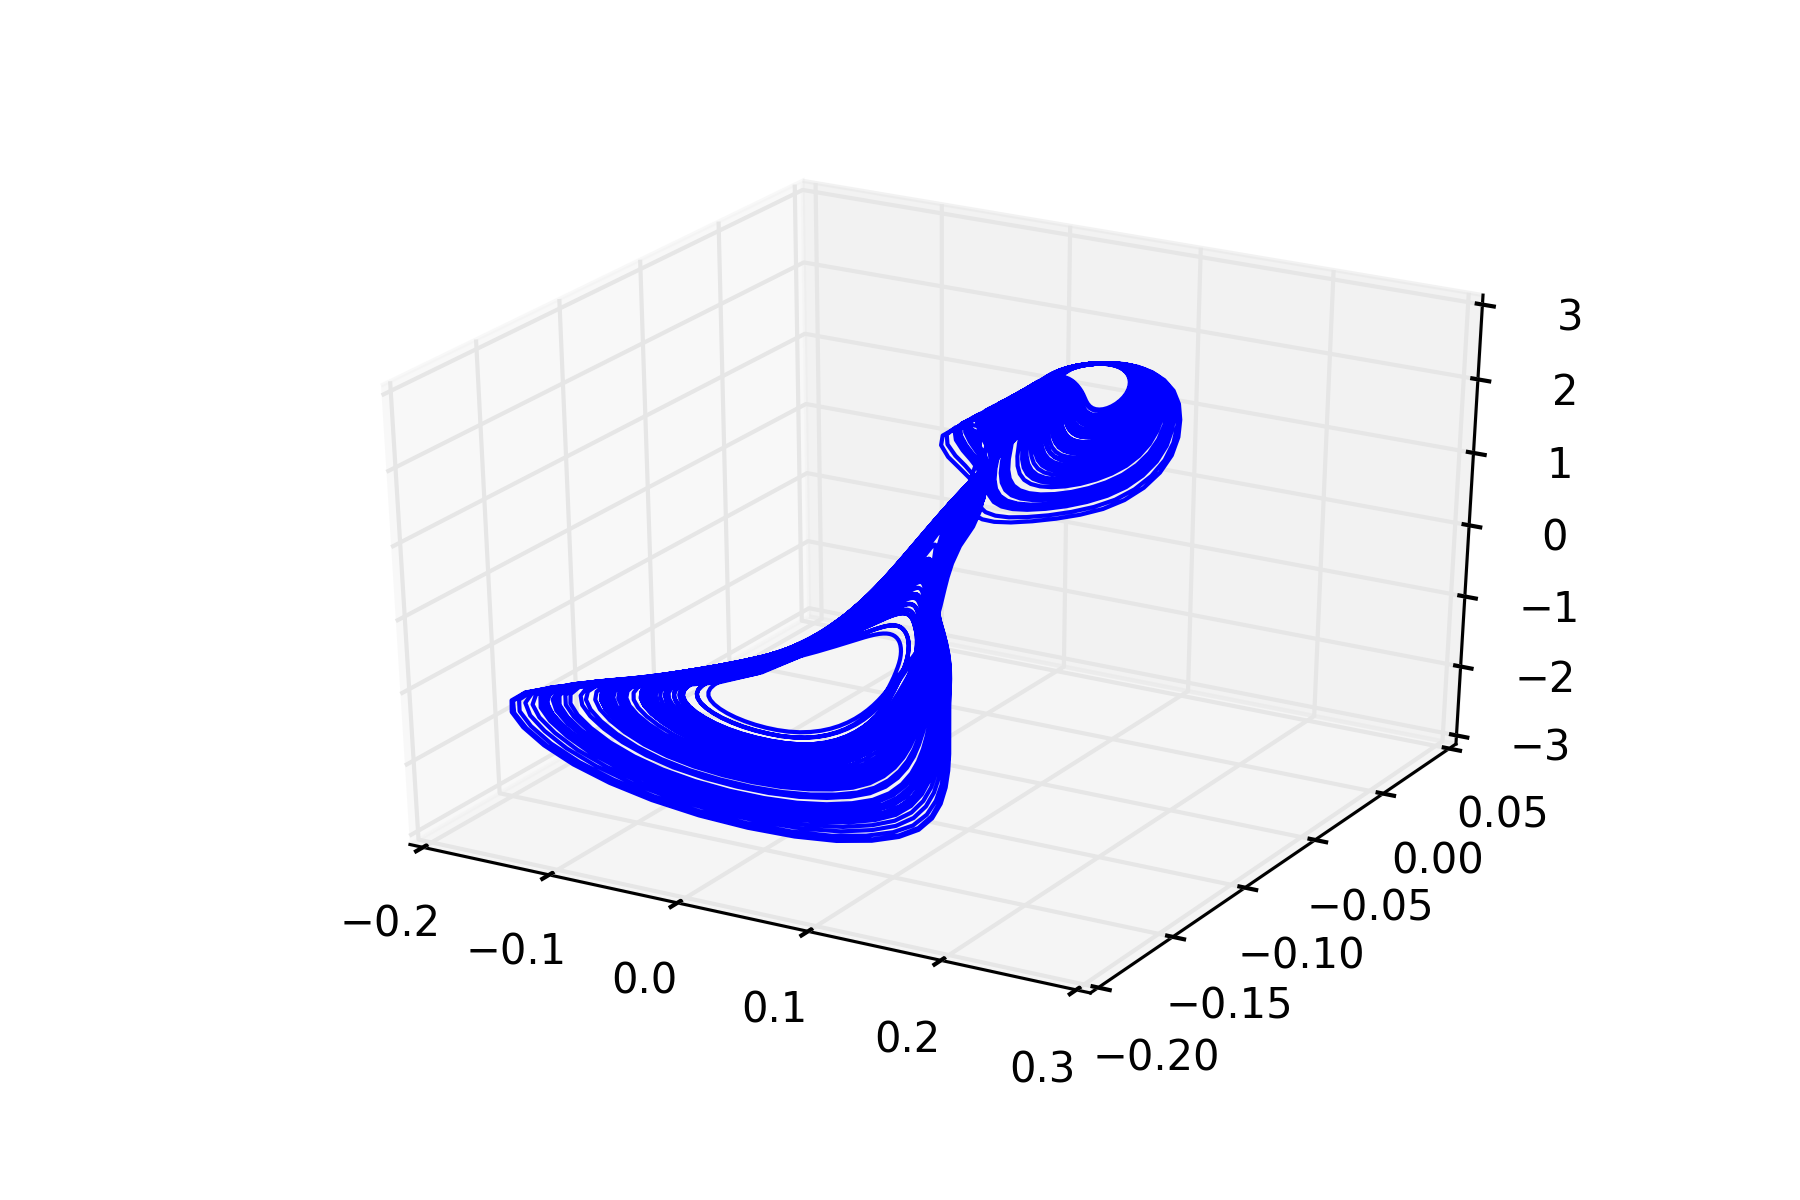
\includegraphics[width=\textwidth]{attractor6}
			\end{minipage}
			\hfill
			\begin{minipage}{0.45\textwidth}
				\centering
				Dimensionality of the latent space?
				\begin{equation*}
				\begin{aligned}
					d_E &\sim \q{d_E}{\bxTs}{\phi}\\
					f_{d_E} &: \RR^N \to \RR^{d_E}\\
					f_{d_E} &: \bxTs \mapsto \bzTs
				\end{aligned}
				\end{equation*}
			\end{minipage}
		\end{figure}
	\end{frame}

\section{Why do we need this?}

		\begin{frame}{General Computation Graph}
		\begin{figure}
			\centering
			\begin{tikzpicture}
			\node (inpt) at (0, 0) {$\bx$};
			
			\layer{inpt}{0}{0};
			\layer{a0}{2.5}{1};
			\layer{a1}{5}{2};
			
			\node[draw, right = .5 of a2] (loss) {$\loss{\ba^{(2)}, \by}$};
			\draw[->] (a2) to (loss);
			\end{tikzpicture}
		\end{figure}
	\end{frame}

	\begin{frame}{Backprop Equations}
		Let $\delta^{(l)} = \frac{ \partial \loss{\cdot} }{ \partial \bz^{(l)}}$, then backprop is given by:
		\begin{equation}
			\delta^{(L)} = \nabla_{\ba^{(L)}} \loss{\ba^{(L)}, \by} \odot \sigma' \left( \bz^{(L)} \right),
		\end{equation} 
		\begin{equation}
			\delta^{(l)} = \left( \left( \bW^{(l+1)} \right)^T \delta^{(l+1)} \right) \odot \sigma' \left( \bz^{(l)} \right),
		\end{equation}
		\begin{equation}
			\frac{\partial \loss{\cdot} }{\partial \bW^{(l)} }   = \delta^{(l)}  \left( \ba^{(l-1) } \right)^T.
		\end{equation}
	\end{frame}
	
	
	\begin{frame}{Stochastic Computation Graph}
		\begin{figure}
			\centering
			\begin{tikzpicture}
			\node (inpt) at (0, 0) {$\bx$};
			
				\layer{inpt}{0}{0};
				\layer[$\p{\bx}$] {a0}{2.5}{1};
				\layer[$1$]{a1}{5}{2};
				
				\node[draw, right = .5 of a2] (loss) {$\frac{1}{2} \left(\by - \ba^{(2)} \right)^2$};
				\draw[->] (a2) to (loss);
			\end{tikzpicture}
		\end{figure}
	\end{frame}

	\begin{frame}{Forward pass}
		\begin{equation*}
			\begin{aligned}
				\bz\idx{0} &= \bW\idx{0} \bx\\
				\uncover<2->{\ba\idx{0} &= \sigma \left( \bz\idx{0} \right)}\\
				\uncover<3->{\bz\idx{1} &= \bW\idx{1} \ba\idx{1}}\\
				\uncover<4->{\theta &= \sigma \left( \bz\idx{1} \right)}\\
				\uncover<5->{\ba\idx{1} &\sim \p{\ba}{\theta}}\\
				\uncover<6->{\bz\idx{2} &= \bW\idx{2} \ba\idx{1}}\\
				\uncover<7->{\ba\idx{2} &= \bz\idx{2}}\\
				\uncover<8->{\loss{\cdot} &= \frac{1}{2} \left( \by - \ba\idx{2} \right)^2}\\
			\end{aligned}
		\end{equation*}
	\end{frame}

	\begin{frame}{Backward pass}
		\begin{equation*}
		\begin{aligned}
			\bz\idx{0} &= \bW\idx{0}\bx\\
			\ba\idx{0} &= \sigma \left( \bz\idx{0} \right)\\
			\bz\idx{1} &= \bW\idx{1} \ba\idx{1} & \uncover<3->{\vdots}\\
			\theta &= \sigma \left( \bz\idx{1} \right)\\
			\ba\idx{1} &\sim \p{\ba}{\theta} & \uncover<3->{     \delta\idx{1} =  \left( \left( \bW\idx{2} \right)^T \delta\idx{2} \right)  \odot \textcolor{red} {\frac{ \partial \ba\idx{1} } { \partial \bz\idx{1} }} }\\
			\bz\idx{2} &= \bW\idx{2} \ba\idx{1} \\
			\ba\idx{2} &= \bz\idx{2} \qquad \qquad & \delta\idx{2} = (\by - \ba\idx{2} )\\
			\loss{\cdot} &= \frac{1}{2} \left( \by - \ba\idx{2} \right)^2 \\
		\end{aligned}
		\end{equation*}
	\end{frame}

	\begin{frame}{Gradient of a sample?}
%	It'd be no problem if we were interested in the gradient of a probability of a specific event; it's simple to compute that
%	The problem is, the event we're interested in depends on the probability and is discrete - there's no gradient whatsoever

		\begin{equation}
			\begin{aligned}
				\frac{ \partial \ba\idx{1} } { \partial \bz\idx{1} } &= \frac{ \ba\idx{1} }{ \partial \p{ \ba\idx{1} }{ \theta }}  \frac{ \partial \p{ \ba\idx{1} }{ \theta }}{ \partial \bz\idx{1} } \\
				&= \frac{ \ba\idx{1} }{ \partial \p{ \ba\idx{1} }{ \theta }}  \frac{ \partial \p{ \ba\idx{1} }{ \theta }}{ \partial \theta } \frac{\partial \theta}{\partial \bz\idx{1}}\\
			\end{aligned}
		\end{equation}
		\uncover<2->{
		but...
		\begin{equation}
			\begin{aligned}
				\ba\idx{1} \sim \p{ \ba }{ \theta }\\
				\uncover<3->{\frac{ \ba\idx{1} }{ \partial \p{ \ba\idx{1} }{ \theta }} = \nexists}
			\end{aligned}
		\end{equation}}
		
	\end{frame}
	
\section{Continuous Random Variables: One-Liners}

	\begin{frame}{(Continuous) Reparametrisation Trick}
		Let $\bx \sim \p{\bx}{\theta}$ be a random variable. Perform change of variables such that
		\begin{equation}
			\begin{aligned}
				\epsilon &\sim \p{\epsilon},\\
				\bx &= g( \epsilon, \theta)
			\end{aligned}
		\end{equation}
		and treat $\epsilon$ as if it was a constant.
		
		\uncover<2->{
		Example:
		\begin{equation*}
			\begin{aligned}
				\epsilon &\sim \gauss{0, 1}\\
				x &\sim \gauss{2, \frac{1}{4}} = \gauss{\mu, \sigma^2}\\
				x &= g( \epsilon, \mu, \sigma^2) = \mu + \sigma  \epsilon = 2 + \frac{1}{2} \epsilon\\
			\end{aligned}
		\end{equation*}}
		\uncover<3->{\begin{equation*}
			\frac{\dint x}{\dint \mu} = 1 \qquad\qquad
			\frac{\dint x}{\dint \sigma} = \frac{1}{2} \epsilon \qquad\qquad
			\frac{\dint x}{\dint \epsilon} \overset{!}{=} 0
		\end{equation*}}
	\end{frame}

	\begin{frame}{Why can we do this?}
		\uncover<1-2>{We are NOT computing $\loss{x}$.\\}
		\uncover<2->{We are computing $\nabla_\theta \expc{\loss{x}}{}{\p{x}{\data}{\theta}} = \nabla_\theta \int \p{x}{\data}{\theta} \loss{x} \dint x$.}
		
		\uncover<3->{We get the gradient by the change of variables:
		\begin{equation*}
			\begin{aligned}
				\p{x} &= \abs{ \frac{\dint \epsilon }{ \dint x}} \p{\epsilon}  & \text{Change of variables},\\
				\implies \abs{\p{x} \dint x} &= \abs{ \p{\epsilon} \dint \epsilon} & \text{Mass conservation}.
			\end{aligned}
		\end{equation*}}
	
		\uncover<4->{
		\begin{equation*}
			\begin{aligned}
				&\nabla_\theta \expc{\loss{x}}{}{\p{x}{\data}{\theta} } = \nabla_\theta \int \p{x}{\data}{\theta} \loss{x} \dint x\\
				\uncover<5->{&= \nabla_\theta \int \p{\epsilon} \loss{x} \dint \epsilon}\uncover<6->{= \nabla_\theta \int \p{\epsilon} \loss{g( \epsilon, \theta)} \dint \epsilon\\}
				\uncover<7->{&= \int \p{\epsilon} \nabla_\theta \loss{g( \epsilon, \theta)} \dint \epsilon}\uncover<8->{= \expc{ \nabla_\theta \loss{g( \epsilon, \theta)} }{}{\p{\epsilon}}}
			\end{aligned}
		\end{equation*}}
	\end{frame}

	\begin{frame}{MC approximation}
		How to compute $\expc{ \nabla_\theta \loss{g( \epsilon, \theta)} }{}{\p{\epsilon}}$?
		
		\begin{enumerate}
			\item Sample $\epsilon\idx{s} \sim \p{\epsilon}$.
			\item $\nabla_\theta \loss{x} \simeq \frac{1}{S} \sum_{s=1}^S \nabla_\theta \loss{g( \epsilon\idx{s}, \theta)}$
		\end{enumerate}
	\uncover<2->{\textcolor{red}{What happens to the multiplication by $\p{\cdot}$?}}
	\uncover<3->{
	\begin{equation}
		\expc{ f(x) }{}{\p{x}} = \int\textcolor{red}{ \p{x} } f(x) \dint x \simeq \frac{1}{S} \sum_{s=1}^S  f(x\idx{s})
	\end{equation}}
	\end{frame} 


\section{Discrete Random Variables: REINFORCE}
	\begin{frame}{REINFORCE or the log-derivative trick}
		We can use REINFORCE for continuous variables, too, but one-liners are typically easier and implemented by default.
		
		\vspace{30pt}
		Recall that
		\begin{equation*}
			\nabla \log f(x) = \frac{\nabla f(x)}{f(x)}.
		\end{equation*}
	\end{frame}

	\begin{frame}{REINFORCE}
		Again, we're computing the expectation of the gradient:
		\begin{equation*}
			\begin{aligned}
				\nabla_\theta &\expc{\loss{x}}{}{\p{x}{\data}{\theta}} = \int \nabla_\theta \p{x}{\data}{\theta} \loss{x} \dint x\\
				\uncover<2->{&= \int \frac{\p{x}{\data}{\theta}}{\textcolor{red}{ \p{x}{\data}{\theta} }} \textcolor{red}{\nabla_\theta \p{x}{\data}{\theta}} \loss{x} \dint x}\\
				\uncover<3->{&=\int \p{x}{\data}{\theta} \textcolor{red}{\nabla_\theta \log \p{x}{\data}{\theta}} \loss{x} \dint x}\\
				\uncover<4->{&= \expc{ \nabla_\theta \log \p{x}{\data}{\theta} \loss{x} }{}{\p{x}{\data}{\theta}}}\\
				\uncover<5->{&\simeq \frac{1}{S} \sum_{s=1}^S \nabla_\theta \log \p{x}{\data}{\theta} \loss{x}}
			\end{aligned}
		\end{equation*}
	\end{frame}



\end{document}
  